% =============================================================================
% The LQ Digital Mode Family — Reference Implementation (lq_lib)
%
% Author:  Luis Quesada (HB9IPH)
% Web:     https://luisquesada.com
% Portal:  https://lquesada.github.io/lq_lib/
% GitHub:  https://github.com/lquesada/lq_lib
% App:     qFT8 — Portable Amateur Radio for Android (https://qft8.com)
%
% License: MIT License (https://github.com/lquesada/lq_lib/blob/main/LICENSE)
%
% Copyright (c) 2026 Luis Quesada (HB9IPH)
%
% Permission is hereby granted, free of charge, to any person obtaining a copy
% of this software and associated documentation files (the "Software"), to deal
% in the Software without restriction, including without limitation the rights
% to use, copy, modify, merge, publish, distribute, sublicense, and/or sell
% copies of the Software, and to permit persons to whom the Software is
% furnished to do so, subject to the following conditions:
%
% The above copyright notice and this permission notice shall be included in
% all copies or substantial portions of the Software.
%
% THE SOFTWARE IS PROVIDED "AS IS", WITHOUT WARRANTY OF ANY KIND, EXPRESS OR
% IMPLIED, INCLUDING BUT NOT LIMITED TO THE WARRANTIES OF MERCHANTABILITY,
% FITNESS FOR A PARTICULAR PURPOSE AND NONINFRINGEMENT. IN NO EVENT SHALL THE
% AUTHORS OR COPYRIGHT HOLDERS BE LIABLE FOR ANY CLAIM, DAMAGES OR OTHER
% LIABILITY, WHETHER IN AN ACTION OF CONTRACT, TORT OR OTHERWISE, ARISING FROM,
% OUT OF OR IN CONNECTION WITH THE SOFTWARE OR THE USE OR OTHER DEALINGS IN THE
% SOFTWARE.
% =============================================================================

% ===========================================================================
%  Section IV: Field Encodings (ALLOCATION: PAGE 5)
%  Must fit entirely on Page 5.
%  Terminates with \newpage.
% ===========================================================================

\section{Field Encodings}
\label{sec:fields}
{\setlength{\abovedisplayskip}{2.0pt plus 1.5pt minus 1.0pt}
\setlength{\belowdisplayskip}{2.0pt plus 1.5pt minus 1.0pt}

To maintain compatibility, \LQ{} adopts core field structures from FT8~\cite{ft8,wsjtx} (K9AN/K1JT)---28-bit callsigns, 15-bit grid locators, 20-bit CQ modifiers, and 5-bit signal reports---while introducing 1-bit portable suffixes, Base-38 non-standard callsigns, CRC-24/Q hashes, and a 104-character free-text Varicode.

% -------------------------------------------------------------------
\subsection{Standard Callsign (28 bits)}
\label{sec:std_call}
% -------------------------------------------------------------------

Adopted from FT8~\cite{ft8,wsjtx}, standard ITU amateur callsigns canonicalize to 6 characters anchored around decimal digit $d$ at position~3: $c_1 c_2 d s_1 s_2 s_3$. Prefix ($c_1, c_2$) right-aligns with space padding in $c_1$ if 1 character; suffix ($s_1, s_2, s_3$) left-aligns with spaces. Callsigns matching $c_1 c_2 d s_1 s_2 s_3$ without slashes are standard; all others are non-standard (Section~\ref{sec:nonstd_call}).

Symbol index mappings: $c_1 \in \{\text{\textvisiblespace}, \text{0--9}, \text{A--Z}\}$ (radix 37: space $\to 0$, \texttt{0--9} $\to 1\dots 10$, \texttt{A--Z} $\to 11\dots 36$); $c_2 \in \{\text{0--9}, \text{A--Z}\}$ (radix 36: \texttt{0--9} $\to 0\dots 9$, \texttt{A--Z} $\to 10\dots 35$); $d \in \{\text{0--9}\}$ (radix 10); and $s_1, s_2, s_3 \in \{\text{\textvisiblespace}, \text{A--Z}\}$ (radix 27: space $\to 0$, \texttt{A--Z} $\to 1\dots 26$). With indices $(n_1, \dots, n_6)$, mixed-radix serialization packs into 28-bit integer $N_{28}$:
\begin{equation}
  N_{28} = (n_1 \cdot 36 \cdot 10 + n_2 \cdot 10 + n_3) \cdot 27^3 + n_4 \cdot 27^2 + n_5 \cdot 27 + n_6.
\label{eq:call28}
\end{equation}
Standard callsigns occupy $0 \le N_{28} \le N_{\max} = 262{,}177{,}559 < 2^{28}$; subsequent states encode tokens $\texttt{DE} = 262{,}177{,}560$, $\texttt{QRZ} = 262{,}177{,}561$, and $\texttt{CQ} = 262{,}177{,}562$. Decoders validate radix ranges to reject corrupted values.

% -------------------------------------------------------------------
\subsection{Standard Dedicated Suffixes (1 bit)}
\label{sec:std_portable_suffix}
% -------------------------------------------------------------------

To support field activations (POTA/SOTA) without hashing, frames reserve an explicit 1-bit suffix: \texttt{0}=\emph{none} (e.g., \callsign{HB9IPH}), \texttt{1}=\texttt{/P} (portable).

% -------------------------------------------------------------------
\subsection{Non-Standard Callsigns (Base-38 Big-Integer Packing)}
\label{sec:nonstd_call}
% -------------------------------------------------------------------

Non-standard or slashed callsigns pack as Base-38 strings over alphabet \textvisiblespace{} (0), \texttt{A}--\texttt{Z} (1--26), \texttt{/} (27), and \texttt{0}--\texttt{9} (28--37), right-padded with spaces to length $L$ and evaluated big-endian as $N_{\text{b38}} = \sum_{i=0}^{L-1} v_i \cdot 38^{L-1-i}$. \textbf{9-Char Callsigns (48 bits):} $38^9 < 2^{48}$ (Types 2, 3, 7, 10), supporting up to 9 characters plus 1-bit portable suffix (\texttt{/P}, e.g., \callsign{EA6/HB9IP/P}) or slashed calls (\callsign{HB9IPH/Q}). \textbf{13-Char Callsigns (69 bits):} $38^{13} < 2^{69}$ (Type 4), supporting compound callsigns up to 13 characters plus suffix in CQ (\callsign{3B9/HB9IPH/P}). Unnormalized whitespace is rejected.

\textbf{Alphabet Disambiguation:} This Base-38 alphabet (space $\to 0$, \texttt{A--Z} $\to 1\dots 26$, \texttt{/} $\to 27$, \texttt{0--9} $\to 28\dots 37$) places letters before digits, unlike the legacy WSJT-X order (\texttt{0--9} $\to 1\dots 10$, \texttt{A--Z} $\to 11\dots 36$) used in the 16-bit hash (Section~\ref{sec:hash}).

% -------------------------------------------------------------------
\subsection{Callsign Hashes (24-bit, 20-bit, and 16-bit) \& Dehashing}
\label{sec:hash}
% -------------------------------------------------------------------

Non-standard stations addressed in directed frames are identified via collision-resistant hashes:
\textbf{24-Bit Callsign Hash ($H_{24}$):} Computed over trimmed ASCII callsigns via CRC-24/Q~\cite{crc24q} ($G(x) = \texttt{0x1864CFB}$, init/final \texttt{0x000000}, non-reflected): $H_{24}(\text{call}) = \text{CRC-24/Q}(\text{call})$, yielding $2^{24} = 16{,}777{,}216$ states ($P_{\text{collision}} \le 0.75\%$ across 500 stations).
\textbf{20-Bit Target Hash ($H_{20}$):} Used in Type~7 directed replies as 20 MSBs: $H_{20}(\text{call}) = \lfloor H_{24}(\text{call}) / 2^4 \rfloor = H_{24}(\text{call}) \gg 4$, yielding $2^{20} = 1{,}048{,}576$ states (e.g., $H_{20} = \texttt{0x01A4F}$ for $H_{24} = \texttt{0x01A4F2}$), conserving 4 payload bits for reports while maintaining high collision resistance.

\textbf{16-Bit DX Callsign Hash ($H_{16}$):} Used in multi-station frames (Types 11 and 12), computed via the WSJT-X 16-bit multiplicative hash~\cite{wsjtx}. Callsigns right-pad to 11 characters over alphabet (\textvisiblespace{} $\to 0$, \texttt{0--9} $\to 1\dots 10$, \texttt{A--Z} $\to 11\dots 36$, \texttt{/} $\to 37$):
\begin{equation}
  H_{16}(\text{call}) = \lfloor (\textstyle\sum_{i=0}^{10} v_i \cdot 38^{10-i} \cdot 47055833459) / 2^{48} \rfloor \bmod 2^{16},
\end{equation}
yielding 65,536 states (e.g., $H_{16}(\text{\callsign{HB9IPH}}) = \texttt{0x7A8B}$).

\textbf{UI Resolution:} Resolved hashes display bracketed by callsign (e.g., \texttt{<HB9IPH>}); unresolved hashes display in hex (e.g., \texttt{<01A4F2>}, \texttt{<01A4F>}, or \texttt{<7A8B>}).

% -------------------------------------------------------------------
\subsection{Maidenhead Grid Locator (15 bits)}
\label{sec:locator}

Following the FT8 standard~\cite{ft8,wsjtx,maidenhead}, four-character Maidenhead grid locators ($F_1 F_2 D_1 D_2$, with fields $F_1, F_2 \in [\text{A--R}]$ and squares $D_1, D_2 \in [0\text{--}9]$) divide the globe into $18 \times 18 = 324$ fields of $10 \times 10 = 100$ squares ($32{,}400$ total squares). Packed into 15 bits ($N_{\text{grid}} < 32{,}400 < 2^{15} = 32{,}768$):
\begin{equation}
\begin{aligned}
  N_{\text{grid}} ={}& (F_1 - \text{'A'}) \cdot 1800 + (F_2 - \text{'A'}) \cdot 100 \\
                     & + (D_1 - \text{'0'}) \cdot 10 + (D_2 - \text{'0'}).
\end{aligned}
\label{eq:grid}
\end{equation}
Values $0 \le N_{\text{grid}} \le 32{,}399$ represent valid Maidenhead squares; $N_{\text{grid}} = 32{,}400$ is the blank locator sentinel; values $32{,}401 \le N_{\text{grid}} \le 32{,}767$ are rejected.

% -------------------------------------------------------------------
\subsection{CQ Modifiers (20 bits)}
\label{sec:modifier}
% -------------------------------------------------------------------

Directed CQ frames (Types~1 and 3) adopt the 20-bit modifier structure from WSJT-X / FT8~\cite{ft8,wsjtx} ($2^{20} = 1{,}048{,}576$ states):
\emph{1) Unmodified CQ:} $N_{\text{mod}} = 0$ designates general CQ calls.
\emph{2) 3-Digit Numeric (000--999):} $1 \le N_{\text{mod}} \le 1000$ conveys numeric designators (e.g., net/channel IDs \texttt{CQ 040}), mapped as $N_{\text{mod}} = \text{val} + 1$.
\emph{3) Alphanumeric Tokens ($\le 4$ chars):} $1001 \le N_{\text{mod}} \le 1{,}048{,}575$ encodes tokens up to 4 characters (e.g., \texttt{DX}, \texttt{NA}, \texttt{POTA}, \texttt{SOTA}, \texttt{QRP}, \texttt{CQWW}; values $> 2^{20}-1$ rejected). Tokens $< 4$ characters right-pad with spaces over a 32-symbol alphabet (\textvisiblespace{} $\to 0$, \texttt{A--Z} $\to 1\dots 26$, \texttt{0--4} $\to 27\dots 31$):
\begin{equation}
  N_{\text{mod}} = 1000 + \sum_{i=0}^{3} v_i \cdot 32^{3-i}.
\label{eq:modifier}
\end{equation}
Omitting digits 5--9 ensures $32^4 = 2^{20}$ fits without overflow; longer modifiers use 4-character abbreviations (\texttt{WPX}) or free text.

% -------------------------------------------------------------------
\subsection{Signal Reports (5 bits)}
\label{sec:rst}
% -------------------------------------------------------------------

Following FT8~\cite{ft8}, signal reports convey measured SNR from $-26$\,dB to $+5$\,dB via integer $N_{\text{snr}} = \text{clamp}(\text{SNR}_{\text{dB}} + 26, 0, 31) \in [0, 31]$. In directed \msgtype{CALL} replies (Types~5--7), reports display without prefix (e.g., \texttt{-03}); in acknowledgments (\msgtype{REPORT+73}, Types~8 and 11), \texttt{R} is prepended (e.g., \texttt{R-03}).

% -------------------------------------------------------------------
\subsection{Free-Text Varicode Encoding (73 bits)}
\label{sec:varicode}
% -------------------------------------------------------------------

Unstructured text in Type~13 (\msgtype{FREE TEXT}, 73 payload bits) uses a 104-character prefix code (Table~\ref{tab:varicode})~\cite{varicode} optimized from character frequencies~\cite{lewand}. The alphabet spans uppercase \texttt{A--Z}, digits \texttt{0--9}, space, 32 punctuation symbols, 32 Latin-1 characters (¡--Þ), newline \texttt{\textbackslash{}n}, \lightning{}, and \texttt{[FILL]}. Codewords range from 3 to 18 bits (mean 4.25\,bits/char), conveying \textbf{$\approx$17.2 characters} on average ($+32.3\%$ over conventional 13-character payloads). Unused bits are zero-padded; decoders terminate extraction at the first zero bit without emitting fill tokens.
}

\begin{figure*}[!t]
\centering
\vspace{-4pt}
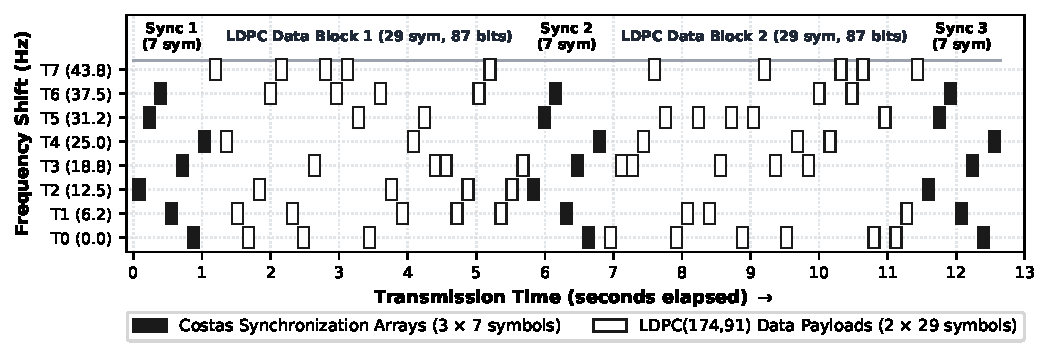
\includegraphics[width=\textwidth]{figures/tones_waterfall_lq8.pdf}
\vspace{-6pt}
\caption{\LQ8 physical frame structure (8-GFSK, 50.0\,Hz bandwidth, 12.64\,s duration).}
\label{fig:waterfall_lq8}
\vspace{-2pt}
\end{figure*}

\pagebreak
